\documentclass[11pt,fancychapters]{article}
\usepackage[a4paper, total={6in, 8in}]{geometry}
\usepackage{cite}
\usepackage{color}
\usepackage{xcolor}
\usepackage{empheq}
\usepackage{setspace}
\usepackage{hyperref}
\usepackage{minted}
\usepackage{acro}
\usepackage{amsmath}
\usepackage{amsthm}
\usepackage{amssymb}
\usepackage{multirow}
\usepackage{graphicx}
\usepackage{geometry}
\usepackage{subcaption}
\usepackage{cancel}
\usepackage[utf8]{inputenc}
\usepackage[english]{babel}
\usepackage{tcolorbox}
\usepackage{hyperref}
\usepackage{cleveref}
\usepackage{parskip}
\usepackage{tcolorbox}
\usepackage{float}
\usepackage{pgfplots}
 \geometry{
 a4paper,
 total={170mm,257mm},
 left=20mm,
 top=20mm,
 }
\pgfplotsset{width=8cm,compat=1.9}
\newcommand{\dbar}{{d\mkern-7mu\mathchar'26\mkern-2mu}}
\newcommand{\boxedeq}[2]{\begin{empheq}[box={\fboxsep=6pt\fbox}]{align}\label{#1}#2\end{empheq}}
\newcommand{\approptoinn}[2]{\mathrel{\vcenter{
  \offinterlineskip\halign{\hfil$##$\cr
    #1\propto\cr\noalign{\kern2pt}#1\sim\cr\noalign{\kern-2pt}}}}}
\newcommand{\appropto}{\mathpalette\approptoinn\relax}
\def\*#1{\mathbf{#1}}
\def\ab{ab}
\usepackage{tikz}
\usetikzlibrary{calc,trees,positioning,arrows,chains,shapes.geometric,%
    decorations.pathreplacing,decorations.pathmorphing,shapes,%
    matrix,shapes.symbols}
\geometry{top=1.3in,bottom=1.3in}

\begin{document}
\centerline{\huge{SUTD ISTD 2021 50.034 Problem Set}}

\begin{table}[ht]
\centering
\footnotesize
 \begin{tabular}{c} 
James Raphael Tiovalen
 \end{tabular}
\end{table}

\section*{Step 1}

\subsection*{Question 1a}

Based on Example 7.6.9 from the course textbook, we have these equations as the method of moments estimators:

\begin{equation}\label{eqn1a1}
    \widehat{\alpha} = \frac{m_1^2}{m_2 - m_1^2}, ~
    \widehat{\beta} = \frac{m_1}{m_2 - m_1^2},
\end{equation}

where $m_1 = \frac{1}{n} \sum_{i=1}^n X_i = \mathbb{E}[X]$ is the sample mean and $m_2 - m_1^2 = \left[ \frac{1}{n} \sum_{i=1}^n X_i^2 \right] - \left[ \frac{1}{n} \sum_{i=1}^n X_i \right]^2 = \mathbb{E}[X^2] - (\mathbb{E}[X])^2$ is the sample variance.\newline

Hence, given that the sample mean and sample standard deviation of $G_\text{SARS}$ are $8.4$ and $3.8$ respectively, we can obtain the method of moments estimates for $\alpha_\text{SARS}$ and $\beta_\text{SARS}$:

\begin{tcolorbox}
\begin{equation}\label{eqn1a2}
    \therefore \widehat{\alpha}_\text{SARS} = \frac{8.4^2}{3.8} = \frac{1764}{95} \approx 18.568, ~
    \widehat{\beta}_\text{SARS} = \frac{8.4}{3.8} = \frac{42}{19} \approx 2.211.
\end{equation}
\end{tcolorbox}

\subsection*{Question 1b}

Modifying Example 7.6.4 from the course textbook accordingly, since both parameters $\alpha$ and $\beta$ are unknown and we would like to estimate both parameters, we use the original p.d.f. of the Gamma distribution:

\begin{equation}\label{eqn1b1}
    f(x) = {\begin{cases}{\frac {\beta^\alpha}{\Gamma(\alpha)} x^{\alpha - 1} e^{-\beta x},}&\mathrm{if} \ x \geq 0;\\[8pt]0,&\mathrm{if} \ x < 0;\end{cases}}
\end{equation}

for some real numbers $\alpha, \beta > 0$.\newline

The likelihood function would be:

\begin{equation}\label{eqn1b2}
    L(\alpha, \beta) = f_n(\boldsymbol{x}|\alpha, \beta) = \frac {\beta^{n\alpha}}{\Gamma^n(\alpha)} \left( \prod_{i=1}^n x_i \right)^{\alpha - 1} \exp\biggl(\, -\beta \sum_{i=1}^{n} x_i \biggr).
\end{equation}

Hence, the log-likelihood function would be:

\begin{equation}\label{eqn1b3}
   \log{ L(\alpha, \beta)} = \log{f_n(\boldsymbol{x}|\alpha, \beta)} = (\alpha-1) \sum_{i=1}^n \log(x_i) - \beta \sum_{i=1}^{n}x_i + n\alpha \log{(\beta)} - n\log{(\Gamma(\alpha))}.
\end{equation}

The maximum likelihood estimators of $\alpha$ and $\beta$ respectively would be the values of $\alpha$ and $\beta$ that satisfy the following equations respectively:

\begin{equation}\label{eqn1b4}
\begin{split}
    \frac{\partial \log{f_n(\boldsymbol{x}|\alpha, \beta)}}{\partial \alpha} & = 0, \\
    \frac{\partial \log{f_n(\boldsymbol{x}|\alpha, \beta)}}{\partial \beta} & = 0.
\end{split}
\end{equation}

Therefore, we would get:

\begin{equation}\label{eqn1b5}
\begin{split}
    \frac{\Gamma'(\alpha)}{\Gamma(\alpha)} & = \log{(\beta)} + \frac{1}{n} \sum_{i=1}^n \log{(x_i)}, \\
    \widehat{\beta} & = \frac{\widehat{\alpha}}{\frac{1}{n} \sum_{i=1}^n x_n} = \frac{\widehat{\alpha}}{\overline{x}_n}.
\end{split}
\end{equation}

Substituting the M.L.E. of $\beta$ into the first equation containing the digamma function, we would get:

\begin{equation}\label{eqn1b6}
    \frac{\Gamma'(\alpha)}{\Gamma(\alpha)} = \log{(\alpha)} - \log{(\overline{x}_n)} + \frac{1}{n} \sum_{i=1}^n \log{(x_i)}.
\end{equation}

We shall then use Newton's method to numerically compute the maximum likelihood estimates of $\alpha$ and $\beta$. First, following Example 7.6.6 from the course textbook, we get these observed values from the full data available at the appendix:

\begin{equation}\label{eqn1b7}
\begin{split}
    \log \left( \frac{1}{180} \sum_{i=1}^{180} x_i \right) = \log \left( \frac{1518}{180} \right) = \log \left( \frac{253}{30} \right) & \approx 2.132, \\
    \frac{1}{180} \sum_{i=1}^{180} \log{(x_i)} & \approx 2.010.
\end{split}
\end{equation}

Then, using Newton's method, we can iteratively approximate the value of the M.L.E. of $\alpha$. Even though we do not know the value of $\beta_\text{SARS}$ for this case, as per Example 7.6.6, we can still set $\alpha_\text{SARS} \approx \frac{253}{30} \approx 8.433$ as our initial guess, which is actually quite similar to the value from the scientific paper on SARS. Hence, Newton's method updates our initial guess, $\alpha_0$, to:

\begin{equation}\label{eqn1b8}
\begin{split}
    \alpha_1 & = \alpha_0 - \frac{\psi(\alpha_0) - \log{(\alpha_0)} + \log{(\overline{x}_n)} - \frac{1}{n} \sum_{i=1}^n \log{(x_i)}}{\psi'(\alpha_0)} \\
    & \approx \alpha_0 - \frac{\psi(8.433) - \log{(8.433)} + 2.132 - 2.010}{\psi'(8.433)} \\
    & \approx 0.0242.
\end{split}
\end{equation}

where $\psi(\alpha)$ is the digamma function and its derivative, $\psi'(\alpha)$, is the trigamma function.\newline

Continuing Newton's method for 15 more iterations would allow the approximation of $\alpha_\text{SARS}$ to stabilize at around $4.261$. Substituting this value into the equation for the M.L.E. of $\beta_\text{SARS}$, we would be able to get $\beta_\text{SARS} \approx 0.505$.

\begin{tcolorbox}
\begin{equation}\label{eqn1b9}
    \therefore \widehat{\alpha}_\text{SARS} \approx 4.261, ~
    \widehat{\beta}_\text{SARS} \approx 0.505.
\end{equation}
\end{tcolorbox}

To show that they are indeed maximum likelihood estimates of $\alpha$ and $\beta$, we get the corresponding second partial derivatives of the log-likelihood function:

\begin{equation}\label{eqn1b10}
\begin{split}
    \frac{\partial^2 \log{f_n(\boldsymbol{x}|\alpha, \beta)}}{\partial \alpha^2} & = -n \psi'(\alpha), \\
    \frac{\partial^2 \log{f_n(\boldsymbol{x}|\alpha, \beta)}}{\partial \beta^2} & = - \frac{n \alpha}{\beta^2}.
\end{split}
\end{equation}

We check that since $\psi'(\alpha) > 0 ~ \forall ~ \alpha \in \mathbb{R}, \alpha > 0$, the second partial derivatives are always negative for all real numbers $\alpha, \beta > 0$. Hence, these are indeed maximum likelihood estimators.

\subsection*{Question 1c}

For a Gamma random variable $X$, we know that $\mathbb{E}[X] = \frac{\alpha}{\beta}$ and $\operatorname{Var}(X) = \frac{\alpha}{\beta^2}$. Hence, the coefficient of variation of a Gamma random variable would be:

\begin{equation}\label{eqn1c1}
    \frac{\sigma}{\left| \mu \right|} = \frac{\sqrt{\alpha}}{\alpha} = \frac{1}{\sqrt{\alpha}}.
\end{equation}

Hence, if $G_\text{SARS}$ and $G_\text{COVID}$ have the same coefficient of variation, this would imply that they have the same value of $\frac{1}{\sqrt{\alpha}}$, and extending this notion by the same vein, the same value of $\alpha$. Therefore, this assumption would imply that $\alpha_\text{SARS} = \alpha_\text{COVID}$.

\subsection*{Question 1d}

\begin{figure}[H]\label{fig:gamma_parameters}
\centering
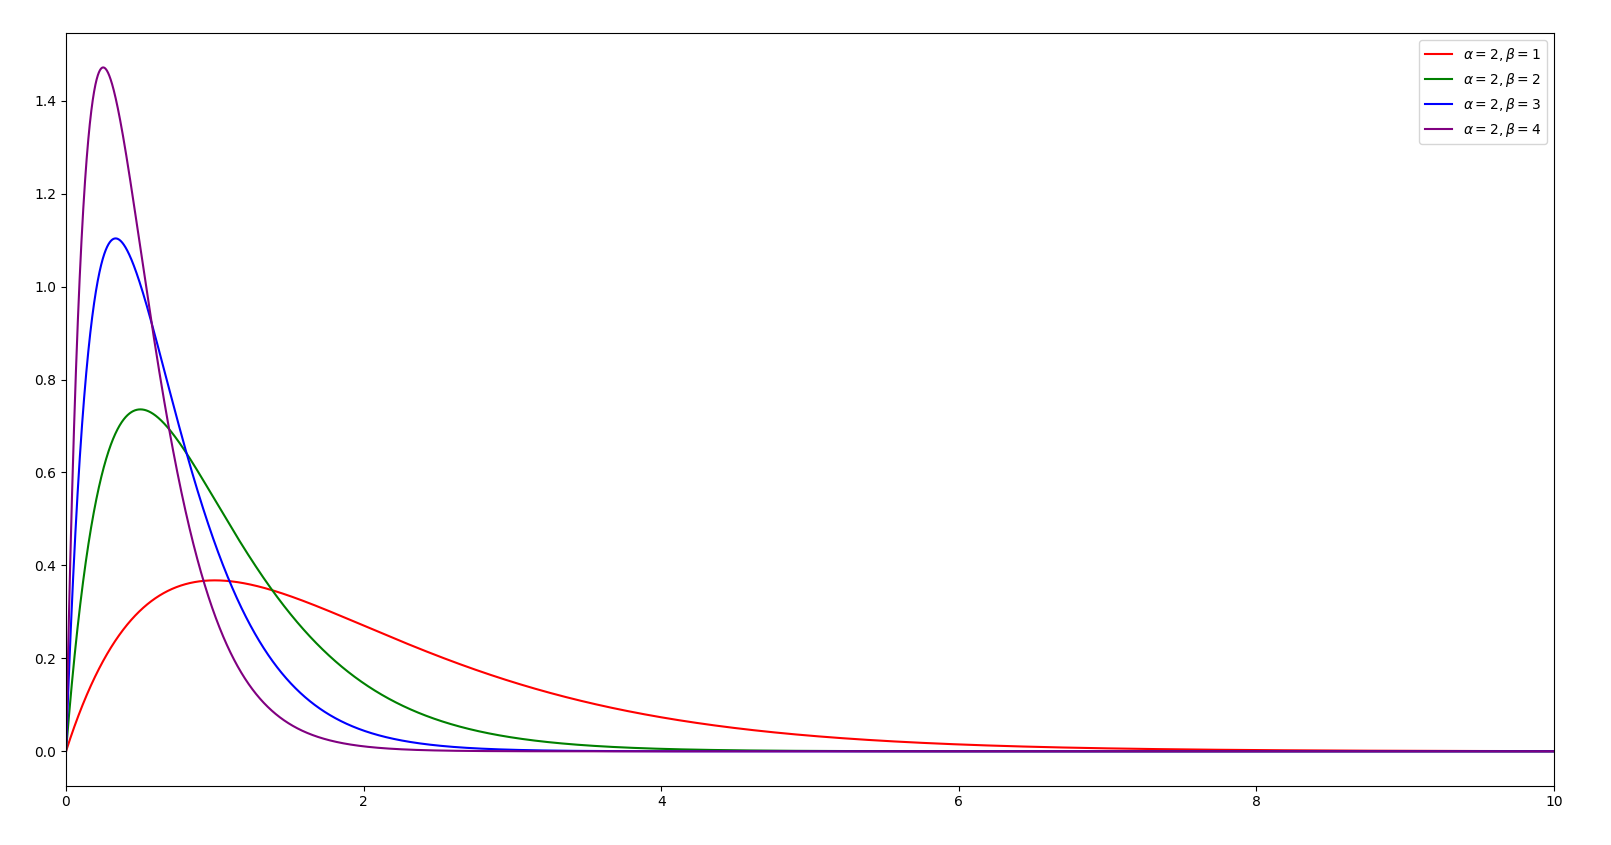
\includegraphics[width=.9\textwidth]{diagrams/gamma.png}
\caption{Probability density function of Gamma distribution for different parameters.}
\label{fig:gamma_graph}
\end{figure}

As the value of $\theta$ increases, the shapes of the graphs become taller and steeper (more concentrated about the mean near zero). More formally, it becomes more positively skewed and more leptokurtic.

\subsection*{Question 1e}

We are given the desired condition that, given that the prior of $\beta_\text{COVID}$ follows a Gamma distribution with prior hyperparameters $2$ and $\lambda$, we want:

\begin{equation}\label{eqn1e1}
    \mathbb{E}\left[ \frac{\alpha_\text{COVID}}{\beta_\text{COVID}} \right] = 8.4.
\end{equation}

Since we can assume that $\alpha_\text{COVID} = \frac{1764}{95}$ is a fixed constant, we can then find the conditional expectation by performing some simple integration:

\begin{equation}\label{eqn1e2}
\begin{split}
    \mathbb{E}\left[ \frac{\alpha_\text{COVID}}{\beta_\text{COVID}} \right] & = (\alpha_\text{COVID}) ~ \mathbb{E} \left[ \frac{1}{\beta_\text{COVID}} \right] \\
    & = \frac{1764}{95} \int_{0}^{\infty} \frac{1}{x} \frac{\lambda^2}{\Gamma(2)} x e^{-\lambda x} ~ \,dx \\
    & = \frac{1764 \lambda^2}{95} \int_{0}^{\infty} e^{-\lambda x} ~ \,dx \\
    & = \frac{1764 \lambda^2}{95} \left[ - \frac{e^{-\lambda x}}{\lambda} \right]_0^\infty \\
    & = \frac{1764 \lambda^2}{95} \left( \frac{1}{\lambda} \right) \\
    & = \frac{1764 \lambda}{95} = 8.4.
\end{split}
\end{equation}

Solving the above equation, we would then obtain:

\begin{tcolorbox}
\begin{equation}\label{eqn1e3}
    \therefore \lambda = \frac{19}{42} \approx 0.452.
\end{equation}
\end{tcolorbox}

\section*{Step 2}

\subsection*{Question 2a}

To infer the observed values for the generation interval $G_\text{COVID}$, we would need to find infected cases for which MOH has provided sufficient information, namely, the links of contact between specific cases. Hence, we need to comb through the multiple Annex C of MOH press releases under the News Highlights section. We only focus on the cases during September 2020 since for this problem set, we mainly aim to study the early exponential growth stage of the COVID-19 epidemic. This is because from October 2020 onwards, the number of cases decreased dramatically. As such, we have obtained several observed values for $G_\text{COVID}$:

\begin{center}
\begin{tabular}{ ||c|c|c|| } 
\hline
Infectee Case Number & Infector Case Number & $G_\text{COVID}$ \\ 
\hline\hline
57186 & 57145 & 1 \\
\hline
57272 & 57145 & 2 \\
\hline
57312 & 57145 & 2 \\
\hline
57322 & 57026 & 7 \\
\hline
57461 & 56190 & 22 \\
\hline
57470 & 57170 & 4 \\
\hline
57513 & 57468 & 1 \\
\hline
57533 & 57453 & 1 \\
\hline
57537 & 57429 & 3 \\
\hline
57551 & 57468 & 1 \\
\hline
57555 & 57428 & 3 \\
\hline
57609 & 57422 & 4 \\
\hline
57638 & 57613 & 1 \\
\hline
57706 & 57689 & 1 \\
\hline
57727 & 57689 & 2 \\
\hline
57728 & 57689 & 2 \\
\hline
57857 & 57829 & 2 \\
\hline
57858 & 57829 & 2 \\
\hline
57867 & 57847 & 1 \\
\hline
57911 & 57847 & 3 \\
\hline
57897 & 57652 & 13 \\
\hline
57915 & 57613 & 16 \\
\hline
57920 & 57870 & 2 \\
\hline
57933 & 57860 & 4 \\
\hline
57939 & 57878 & 3 \\
\hline
57940 & 57927 & 1 \\
\hline
57945 & 57890 & 1 \\
\hline
\end{tabular}
\end{center}

The observed values of $G_\text{COVID}$ are calculated from the time difference between the dates of confirmation of infection between the infector and the infectee. If there are multiple contacts listed under the links entry for the same case, we take the earliest case as the infector. We do not use the symptom onset dates/times since pre-symptomatic transmission is actually possible, and there are plenty of asymptomatic cases in the data. We also conveniently ignore data values with an observed value of $G_\text{COVID}$ of $0$ since those are quite vague since there might be no causal relationship if the generation interval is $0$ days, as well as a little bit complicated since in the calculation that we would need to conduct later, it would just make everything becomes zero.

\subsection*{Question 2b}

We consider a statistical model consisting of $n$ latent continuous random variables $G_1, \dots, G_n$ that are conditionally i.i.d. given the parameter $\theta$. Each $G_i$ represents the generation interval of COVID-19, i.e., the duration (in number of days) from the day the infected individual gets infected, to the day the infected individual infects another individual, whom we will consider to be the $i$-th individual. We get the observed values of $G_i$ by inferring them from the time interval between said infectee is confirmed to be infected by their corresponding infector and the date of confirmation of infection of their infector. Each $G_i$ follows a Gamma distribution with parameters $\alpha_0$ and $\theta$, where $\alpha_0$ is a fixed known constant of around $\frac{1764}{95}$ and $\theta$ is a random variable that follows a prior Gamma distribution with prior hyperparameters $2$ and $\frac{19}{42}$.

\subsection*{Question 2c}

We are given that the prior probability distribution of $\beta_\text{COVID}$ is a Gamma distribution with hyperparameters $\alpha = 2$ and $\beta = \frac{19}{42}$. Let $\boldsymbol{g} = (g_1, \dots, g_{27})$ be the vector of observed values for $(G_1, \dots, G_{27})$, and from Question 2a, we have $g_1 + \dots + g_{27} = 105$ and $n = 27$. Hence, by the given theorem, the posterior distribution of $\beta_\text{COVID}$ is also a Gamma distribution with hyperparameters $\alpha' = \alpha + n\alpha_0 = 2 + (27)(\frac{1764}{95}) = \frac{47818}{95} \approx 503.347$ and $\beta' = \beta + (g_1 + \dots + g_{27}) = \frac{19}{42} + 105 = \frac{4429}{42} \approx 105.452$. Thus, the posterior p.d.f. of $\beta_\text{COVID}$ would be:

\begin{tcolorbox}
\begin{equation}\label{eqn2c1}
    \therefore \xi(\beta | \boldsymbol{g}) = {\begin{cases}{\frac {\left(\frac{4429}{42}\right)^{\frac{47818}{95}}}{\Gamma \left(\frac{47818}{95}\right)} \beta^{\frac{47818}{95} - 1} e^{-\frac{4429}{42} \beta} \approx (7.496 \times 10^{-123}) \beta^{502.347} e^{-105.452 \beta} ,}&\mathrm{if} \ \beta \geq 0;\\[8pt]0,&\mathrm{if} \ \beta < 0.\end{cases}}
\end{equation}
\end{tcolorbox}

\subsection*{Question 2d}

We are given that the prior p.d.f. of $\beta_\text{COVID}$ is:

\begin{equation}\label{eqn2d1}
    \xi(\beta) = {\begin{cases}{\left(\frac{19}{42}\right)^2\beta e^{-\frac{19}{42} \beta},}&\mathrm{if} \ \beta \geq 0;\\[8pt]0,&\mathrm{if} \ \beta < 0.\end{cases}}
\end{equation}

Let $\boldsymbol{g} = (g_1, \dots, g_{27})$ be the vector of observed values for $(G_1, \dots, G_{27})$ obtained in Question 2a. Since $(G_1, \dots, G_{27})$ are continuous, it follows from Bayes' theorem that the posterior p.d.f. of $\beta_\text{COVID}$ is:

\begin{equation}\label{eqn2d2}
    \xi(\beta | \boldsymbol{g}) = \frac{f(\boldsymbol{g} | \beta) \xi(\beta)}{f(\boldsymbol{g})} = \frac{f(\boldsymbol{g} | \beta) \xi(\beta)}{\int_\Omega f(\boldsymbol{g} | \beta') \xi(\beta') \, d\beta'} ~ \mathrm{(for} \ \beta \in \Omega\mathrm{)}.
\end{equation}

Since each $G_i$ is Gamma, the marginal conditional p.d.f. of $G_i$ given $\beta$ is:

\begin{equation}\label{eqn2d3}
    f(g_i | \beta) = {\begin{cases}{\frac{\beta^\frac{1764}{95}}{\Gamma \left( \frac{1764}{95} \right)} g_i^{\frac{1764}{95} - 1} e^{-\beta g_i},}&\mathrm{if} \ g_i \geq 0;\\[8pt]0,&\mathrm{if} \ g_i < 0.\end{cases}}
\end{equation}

Hence, we can compute the likelihood function of $\beta_\text{COVID}$ as follows:

\begin{equation}\label{eqn2d4}
    f(\boldsymbol{g} | \beta) = \frac{\beta^{\frac{47628}{95}}}{\Gamma^{27} \left( \frac{1764}{95} \right)} \left( 21254897664 \right)^{\frac{1764}{95} - 1} e^{-105 \beta} \approx (2.360 \times 10^{-231}) \beta^{501.347} e^{-105 \beta}.
\end{equation}

Therefore, the posterior p.d.f. of $\beta_\text{COVID}$ is:

\begin{equation}\label{eqn2d5}
\begin{split}
    \xi(\beta | \boldsymbol{g}) & = \frac{f(\boldsymbol{g} | \beta) \xi(\beta)}{f(\boldsymbol{g})} \\
    & \approx \frac{(4.830 \times 10^{-232}) \beta^{502.437} e^{-105.452 \beta}}{\int_0^\infty (4.830 \times 10^{-232}) t^{502.437} e^{-105.452 t} \, dt} \\
    & \approx (7.496 \times 10^{-123}) \beta^{502.347} e^{-105.452 \beta},
\end{split}
\end{equation}

which is the same posterior p.d.f. as the one obtained in Question 2c.

\subsection*{Question 2e}

For sensitivity analysis, we vary the value of $\lambda$ and check how the output varies. Based on the theorem specified in the problem set, we know that the value of the posterior $\alpha$ hyperparameter would not change or be affected by any changes in the value of $\lambda$. Hence, we can instead see how the value of the posterior $\beta$ hyperparameter would change. Since $\beta$ is the rate parameter of the Gamma distribution, we can decide to vary the value of $\lambda$ to arbitrarily take in values in the interval $(0, 4]$ at $0.01$ interval hop units. The reason for this is because we do not expect the value of the rate parameter itself of the generation interval of COVID-19 to vary greatly, especially since we consider a small time window interval of only the early stages of the epidemic. We do not select any values of $\lambda \leq 0$ since the definition of a Gamma p.d.f. requires $\lambda > 0$.\newline

By plotting the resulting posterior Gamma distributions of $\beta_\text{COVID}$ as the value of $\lambda$ is varied, we can see how sensitive the value of $\beta_\text{COVID}$ is with respect to the value of $\lambda$:

\begin{figure}[H]\label{fig:normal_sensitivity}
\centering
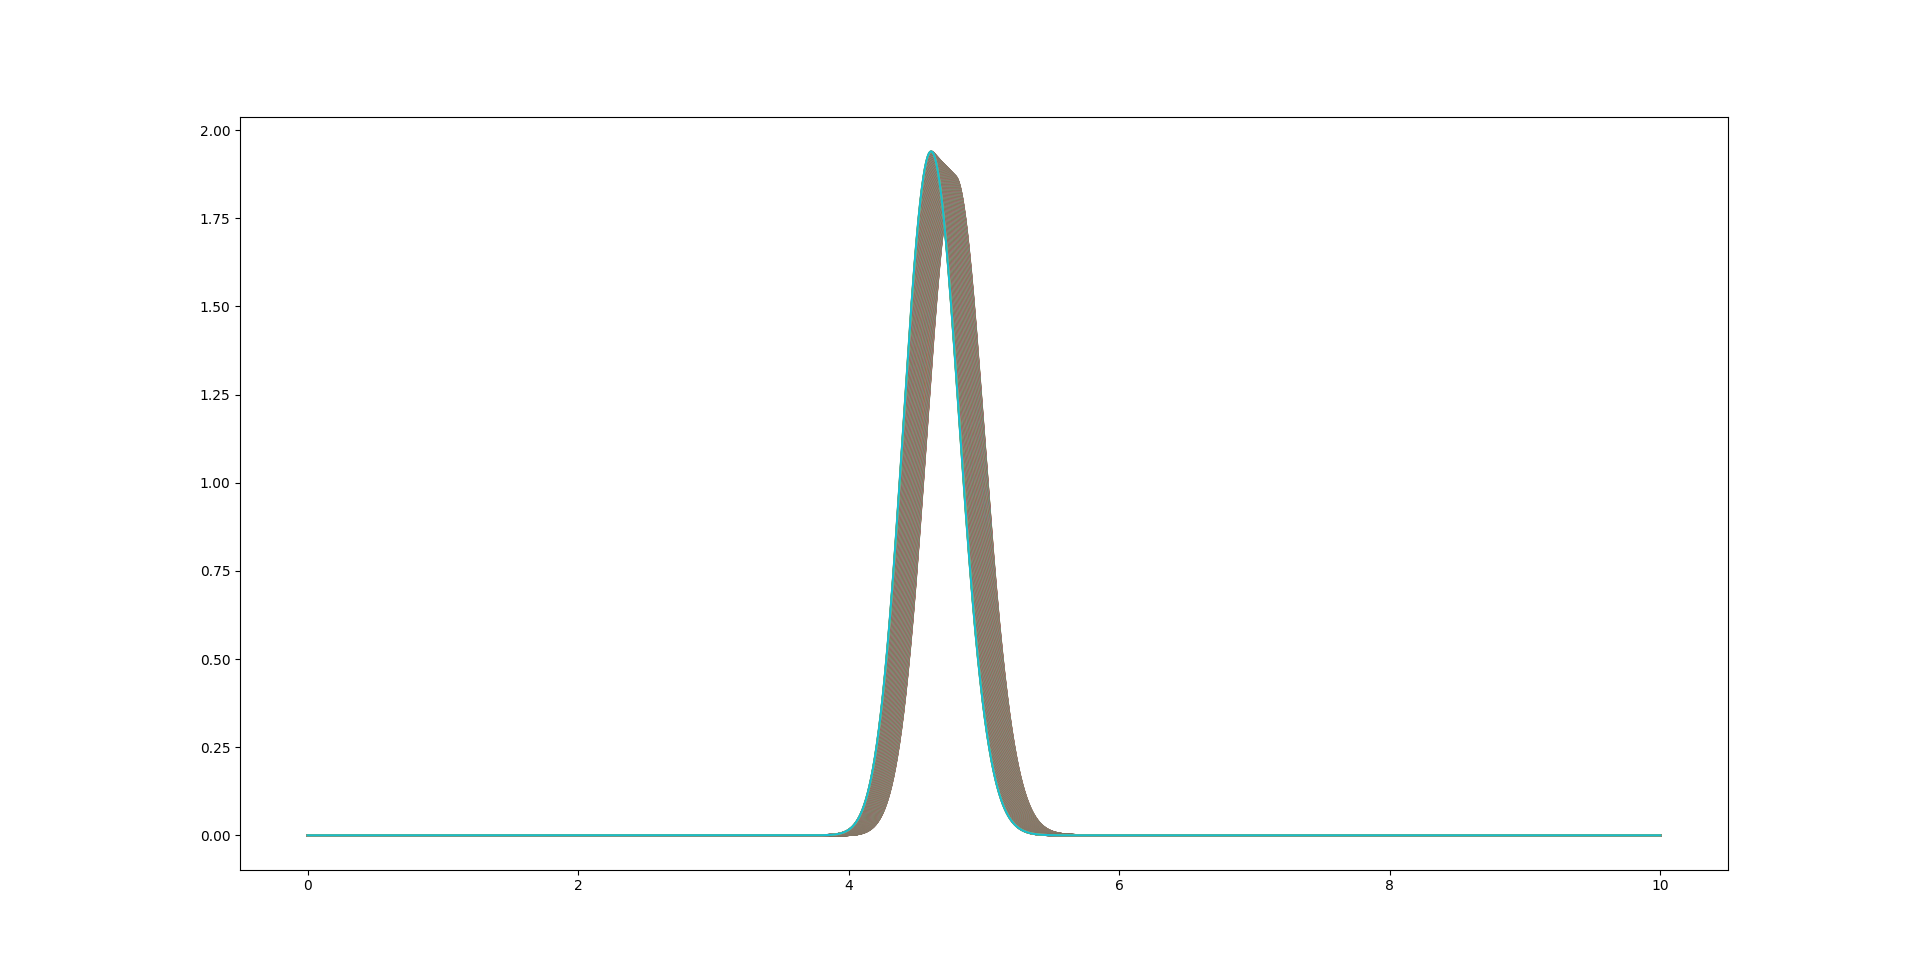
\includegraphics[width=.9\textwidth]{diagrams/normal_sensitivity.png}
\caption{Sensitivity of the posterior Gamma distribution of $\beta_\text{COVID}$ as $\lambda$ varies in $(0, 4]$.}
\label{fig:normal_sensitivity_graph}
\end{figure}

As seen from the diagram above, the posterior mean of $\beta_\text{COVID}$ is relatively stable and consistent at around $4.773$.

In contrast, if we plot the resulting posterior Gamma distributions of $\beta_\text{COVID}$ as the value of $\lambda$ is varied in a different interval, let's say for example in the interval $[0.5, 100.5]$ at $1$ interval hop units, we get this result:

\begin{figure}[H]\label{fig:large_sensitivity}
\centering
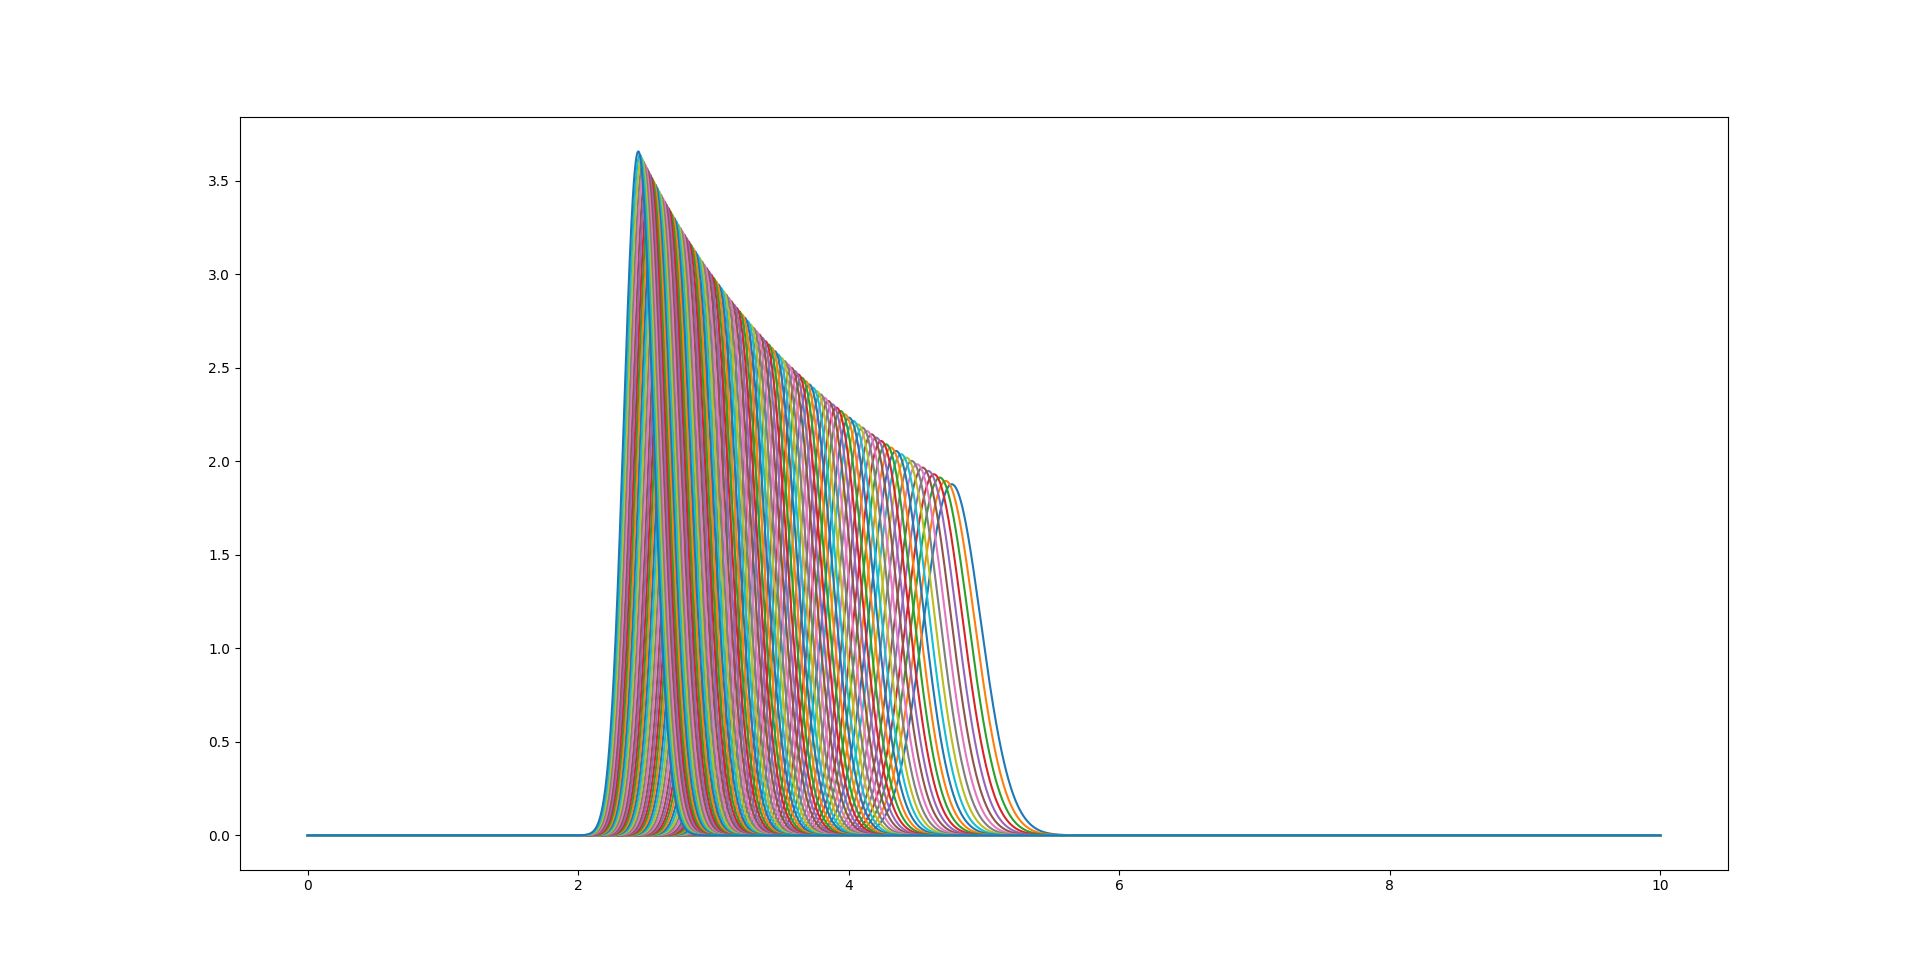
\includegraphics[width=.9\textwidth]{diagrams/large_sensitivity.png}
\caption{Sensitivity of the posterior Gamma distribution of $\beta_\text{COVID}$ as $\lambda$ varies in $(0, 100]$.}
\label{fig:large_sensitivity_graph}
\end{figure}

As seen from the two diagrams, we can see that generally, the mean or expected value of $\beta_\text{COVID}$ decreases as $\lambda$ increases.

\section*{Step 3}

\subsection*{Question 3a}

If the number of COVID-19 cases has an exponential growth over time, this would imply that the number of infected cases on Day $k$ equals approximately:

\begin{equation}\label{eqn3a1}
    n_k = n_0 e^{rk},
\end{equation}

where $n_0$ represents the number of infected cases on Day $0$.\newline

Since $z_k$ is the cumulative number of COVID-19 cases in the United States from Day $0$ to Day $k$ inclusive, we would also get:

\begin{equation}\label{eqn3a2}
    z_k = z_0 e^{rk},
\end{equation}

Even if $z_k$ is discrete, the equation above still shows that $z_k \appropto e^k$. Hence, since $y_k = \ln{z_k}$:

\begin{equation}\label{eqn3a3}
    y_k = \ln{z_0} + rk,
\end{equation}

which shows that $y_k \propto k$. Therefore, $y_k$ grows linearly with respect to $k$.

\subsection*{Question 3b}

By processing the data, we get:

\begin{center}
\begin{tabular}{ ||c|c|c|| } 
\hline
$x_k$ & $z_k$ & $y_k$ \\ 
\hline\hline
1 & 69 & 4.234 \\
2 & 89 & 4.489 \\
3 & 103 & 4.635 \\
4 & 125 & 4.828 \\
5 & 159 & 5.069 \\
6 & 233 & 5.451 \\
7 & 338 & 5.823 \\
8 & 433 & 6.071 \\
9 & 554 & 6.317 \\
10 & 754 & 6.625 \\
11 & 1025 & 6.932 \\
12 & 1312 & 7.179 \\
13 & 1663 & 7.416 \\
14 & 2174 & 7.684 \\
15 & 2951 & 7.990 \\
16 & 3774 & 8.236 \\
17 & 4661 & 8.447 \\
18 & 6427 & 8.768 \\
19 & 9415 & 9.150 \\
20 & 14250 & 9.565 \\
21 & 19624 & 9.885 \\
22 & 26747 & 10.194 \\
23 & 35206 & 10.469 \\
24 & 46442 & 10.746 \\
25 & 55231 & 10.919 \\
26 & 69194 & 11.145 \\
27 & 85991 & 11.362 \\
28 & 104686 & 11.559 \\
29 & 124665 & 11.733 \\
30 & 143025 & 11.871 \\
31 & 164620 & 12.011 \\
\hline
\end{tabular}
\end{center}

By performing linear regression with a least-squares method on the collected data above, we would be able to get the value of $r$ from the gradient and the value of $\ln{z_0}$ from the $y$-intercept:

\begin{tcolorbox}
\begin{equation}\label{eqn3b1}
    \therefore r \approx 0.276, ~
    z_0 \approx 47.659.
\end{equation}
\end{tcolorbox}

\section*{Step 4}

\subsection*{Question 4a}

Since we have the values of $\alpha_\text{COVID} = \frac{1764}{95} \approx 18.568$, $\beta_\text{COVID} \approx 4.773$ and $r \approx 0.276$, we can simply substitute all of them into the original equation in the beginning of this problem set to get our approximation of the basic reproduction number of COVID-19, $R_0$, to be:

\begin{tcolorbox}
\begin{equation}\label{eqn4a1}
    \therefore R_0 \approx \left( 1 + \frac{r}{\beta_\text{COVID}} \right)^{\alpha_\text{COVID}} \approx 2.842.
\end{equation}
\end{tcolorbox}

\subsection*{Question 4b}

Two limitations for the model assumptions that we have employed in this problem set would be:

\begin{enumerate}
    \item The selection of a Gamma probability distribution as the prior distribution of $\beta_\text{COVID}$ might not be appropriate. For all we know, the rate parameter of the generation interval can follow any kind of probability distribution. We simply chose a Gamma prior since it would lead us to relatively nice results/outcomes for the posterior distribution. At the same time, $G_1, \dots, G_n$ might not actually be conditionally i.i.d. in the real-life, since more occurrences of either shorter or longer generation intervals might inevitably and actually affect other observed values of the generation interval, especially if the human population being considered are within close proximity with one another.
    \item The values of $\alpha_\text{COVID}$ and $\alpha_\text{SARS}$ might be different since $G_\text{COVID}$ and $G_\text{SARS}$ might have different coefficients of variation. While COVID-19 and SARS are both caused by coronaviruses, the circumstances surrounding the occurrences of the epidemics are also vastly different. COVID-19 should be able to spread far quicker in this more globalized society in this decade than back in the early 2000s. The lethality rate of COVID-19 is also lower than that of SARS, allowing COVID-19 to continue to spread as the human hosts continue to travel and move around the globe. This would result in a possibly larger value of $R_0$ than the one that we have approximated.
\end{enumerate}

\end{document}
